\chapter{\MakeUppercase{Компьютерное моделирование}}

Зададим наблюдатель, который будет удовлетворять найденным условиям устойчивости:
$$
L=\begin{bmatrix}
    -2 \\ 3
\end{bmatrix}
$$

Воспользуемся программой \textit{Wolfram Mathematica}. Код программы, моделирующей процессы стабилизации системы (1), находится в Приложении Б.

\textbf{1. Задача модальной стабилизации}

Смоделируем процесс стабилизации для случая, когда вектор состояния имеет вид $ u=-kx $, при этом:
$$
k=\begin{bmatrix} 0 & 2 \end{bmatrix}
$$

\begin{figure}[h]
    \centering
    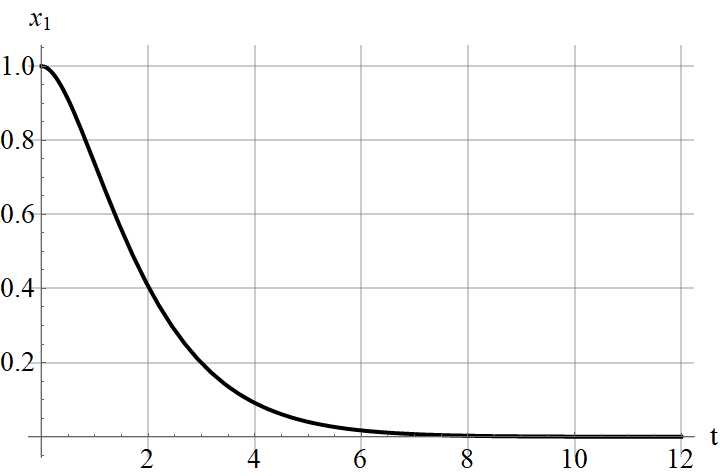
\includegraphics[scale=0.4]{chapter_x6/fig1.png}
    \caption{График $ x_1(t) $}
    \label{1}
\end{figure}


\begin{figure}[h]
    \centering
    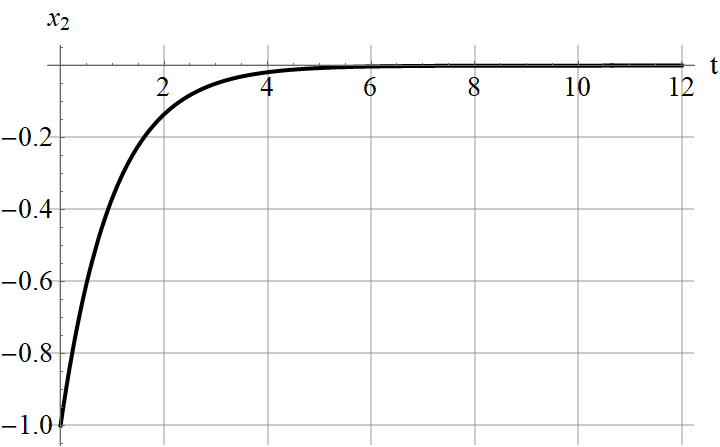
\includegraphics[scale=0.4]{chapter_x6/fig2.png}
    \caption{График $ x_2(t) $ }
    \label{1}
\end{figure}

\newpage

\textbf{2. Линейно-квадратичная задача оптимального управления ($ J_1 $)}

Смоделируем процесс стабилизации для случая, когда вектор состояния имеет вид $ u=-kx $, при этом:
$$
k = \begin{bmatrix} 0 & 2 \end{bmatrix}
$$

Графики построены в следующем пункте.

\textbf{3. Линейно-квадратичная задача оптимального управления ($ J_2 $)}

Смоделируем процесс стабилизации для случая, когда вектор состояния имеет вид $ u=-kx $, при этом:
$$
k = \begin{bmatrix} 1 & 3 \end{bmatrix}
$$

\begin{figure}[h]
    \centering
    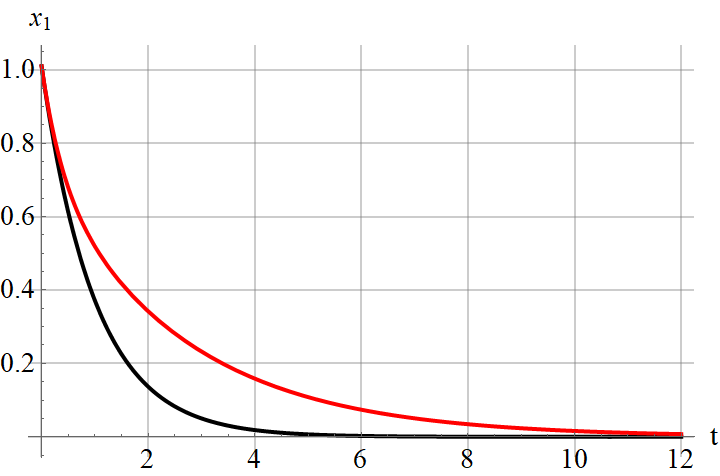
\includegraphics[scale=0.4]{chapter_x6/fig3.png}
    \caption{График $ x_1(t) $ J1 (черный) и $ x_1(t) $ J2 (красный) }
    \label{}
\end{figure}

\begin{figure}[h]
    \centering
    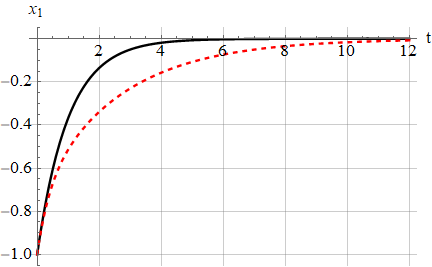
\includegraphics[scale=0.7]{chapter_x6/fig4.png}
    \caption{График $ x_2(t) $ J1 (черный) и $ x_2(t) $ J2 (красный) }
    \label{}
\end{figure}

\newpage

\textbf{4. Линейно-квадратичная задача оптимального управления ($ J_1 $) с ассимптотическим наблюдателем }

Смоделируем процесс стабилизации для случая, когда оценка состояния имеет вид $ u=-k\hat{x} $, при этом $ k $ коэффициент усиления взят из линейно-квадратичной задачи оптимального управления ( $ J_1 $ ):
$$
k = \begin{bmatrix} 0 & 2 \end{bmatrix}
$$

\begin{figure}[h]
    \centering
    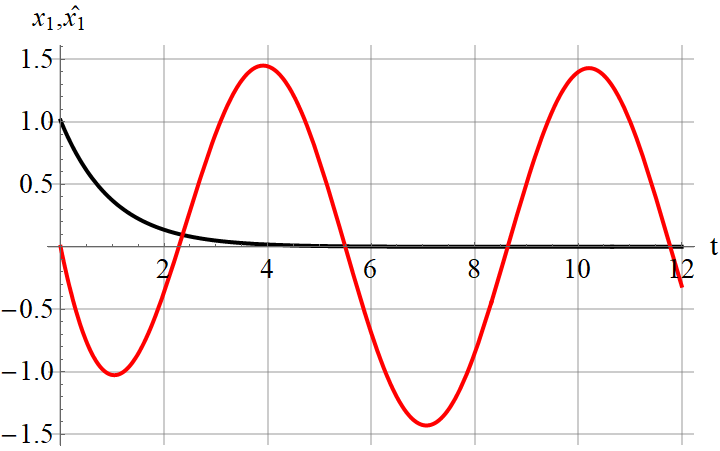
\includegraphics[scale=0.7]{chapter_x6/fig5.png}
    \caption{График $ x_1(t) $ (черный) и $ \hat{x}_1(t) $ (красный)}
    \label{}
\end{figure}

\begin{figure}[h]
    \centering
    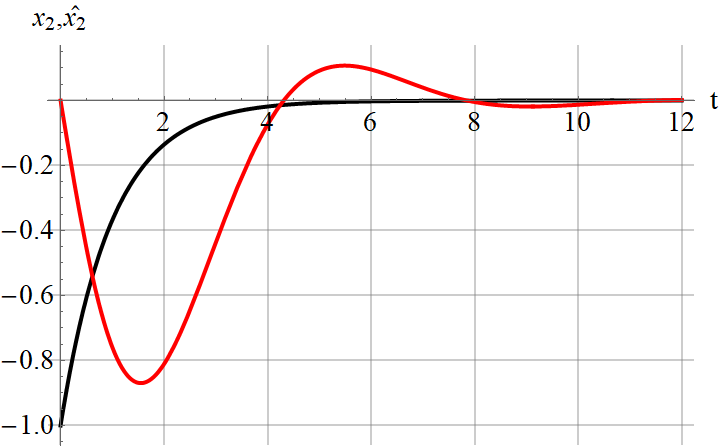
\includegraphics[scale=0.7]{chapter_x6/fig6.png}
    \caption{График $ x_2(t) $ (черный) и $ \hat{x}_2(t) $ (красный)}
    \label{}
\end{figure}